\acresetall
\chapter{Evaluation and Results}\label{ch:evaluation}
In this chapter, a benchmark of the analyzed algorithms is presented, based on dataset size and complexity. For the first part, the algorithms used for supervised learning are presented, for which an analysis of the different complexities used is made. From the benchmark, the trained models with the best performance are saved and then used in the live implementation presented in chapter~\ref{ch:live}. The process of saving trained models for later use is called \emph{model persistence}.

\section{Performance metrics}\label{ch:performance}

The impact of the dataset size on the algorithm performance is of special interest. Given that the data recorded using the procedure described in section~\ref{ch:measure} has a fixed size, this analysis was performed by slicing the resulting feature extraction files to emulate different dataset sizes. It is important to notice that only "slicing", in order to emulate smaller datasets, and not "repeating samples", for emulation of bigger datasets, has a significant impact on the performance, as noted in section~\ref{ch:size}. This is due to the fact that repeated samples present no new information to the model, and there is nothing new to learn from them.

The dataset is, then, sliced into four different sizes:

\begin{itemize}
    \item Small dataset (S): is one fourth (1/4) of the original dataset
    \item Medium dataset (M): is one third (1/3) of the original dataset
    \item Large dataset (L): is half (1/2) of the original dataset
    \item Extra Large dataset (XL): the whole set of features extracted as recorded from the signals over the air.
\end{itemize}

Furthermore, a benchmark of the learning algorithms is made based on variations in their complexities. Each algorithm has different ways to represent its own complexity, and this has a significant impact on its overall performance. The \ac{ML} algorithms used in this analysis are K-nearest neighbors, \ac{SVM} and binary tree classification. Their complexities are set as follows:

\begin{itemize}
    \item K-nearest neighbors: the complexity of this algorithm is set by the amount of neighbors that are considered in order to make a classification decision. For the benchmark, different models were trained using 2, 4, 10 and 50 neighbors.
    \item \ac{SVM}: this algorithm allows the designer to select the type of kernel that is used during the learning process. The function of the kernel is to generate internally non-linear transformations over the input data while still behaving as a linear classificator. For this work, the \ac{RBF} is used as a kernel because of its known good performance on multiclass classification problems at the cost of longer training times. The complexity of this model is then set by providing different values to the 'C' parameter of this \ac{RBF} kernel. This parameter sets the trade off between the proneness of the model to result in an erroneous classification and the simplicity of the decision boundary. For this work, values of C=(1, 1000, 1000000) are given.\todo{changed to gamma, fix accordingly}
    \item Decision Trees: in this model, the complexity is ruled by the depth of the decision branch. Here, depths of 2, 5, 10 and 50 are given.
\end{itemize}

Moreover, it is also interesting to determine how the models behave when the features have been scaled. A first glance at the impact of a scaler is presented by using the StandardScaler() from SKlearn, which simply removes the mean of the features and scales them to unit variance. A side-by-side comparison of model performance when trained with unscaled features vs.scaled features is shown as a result of the benchmark. The results are depicted in Figs~\ref{fig:knn}, \ref{fig:dtc} and \ref{fig:svc}.

\begin{figure}[!htb]
    \centering
    \begin{subfigure}[t]{0.49\textwidth}
        \centering
        \begin{tikzpicture}[scale=0.8]
            \begin{axis}[
                xlabel={\# of Neighbors},
                ylabel={Accuracy},
                legend style={at={(1.2,1.20)},
                    anchor=north,legend columns=-1},
                  ]
                \addplot[color=blue] table [x=N, y=S, col sep=comma, mark=none] {data/knn_accs.csv};
                \addplot[color=red] table [x=N, y=M, col sep=comma, mark=none] {data/knn_accs.csv};
                \addplot[color=green] table [x=N, y=L, col sep=comma, mark=none] {data/knn_accs.csv};
                \addplot[color=orange] table [x=N, y=XL, col sep=comma, mark=none] {data/knn_accs.csv};
                \legend{Dataset S, Dataset M, Dataset L, Dataset XL}
        \end{axis}
        \end{tikzpicture}
        \caption{Accuracy with unscaled features}
        \label{fig:knn_accs_scaled}
    \end{subfigure}
        \hfill
    \begin{subfigure}[t]{0.49\textwidth}
        \centering
        \begin{tikzpicture}[scale=0.8]
            \begin{axis}[
                xlabel={\# of Neighbors},
                ylabel={Accuracy},
                  ]
                \addplot[color=blue] table [x=N, y=S, col sep=comma, mark=none] {data/knn_accs_scaled.csv};
                \addplot[color=red] table [x=N, y=M, col sep=comma, mark=none] {data/knn_accs_scaled.csv};
                \addplot[color=green] table [x=N, y=L, col sep=comma, mark=none] {data/knn_accs_scaled.csv};
                \addplot[color=orange] table [x=N, y=XL, col sep=comma, mark=none] {data/knn_accs_scaled.csv};
                \legend{Dataset S, Dataset M, Dataset L, Dataset XL}
        \end{axis}
        \end{tikzpicture}
        \caption{Accuracy with scaled features}
        \label{fig:knn_accs_scaled}
    \end{subfigure}
    \begin{subfigure}[t]{0.49\textwidth}
        \centering
        \begin{tikzpicture}[scale=0.8]
            \begin{axis}[
                xlabel={\# of Neighbors},
                ylabel={Training time (s)},
                  ]
                \addplot[color=blue]table [x=N, y=S, col sep=comma, mark=none] {data/knn_fit_times.csv};
                \addplot[color=red] table [x=N, y=M, col sep=comma, mark=none] {data/knn_fit_times.csv};
                \addplot[color=green] table [x=N, y=L, col sep=comma, mark=none] {data/knn_fit_times.csv};
                \addplot[color=orange] table [x=N, y=XL, col sep=comma, mark=none] {data/knn_fit_times.csv};
        \end{axis}
        \end{tikzpicture}
        \caption{Training times with unscaled features}
        \label{fig:knn_fit_times}
    \end{subfigure}
    \centering
        \hfill
    \begin{subfigure}[t]{0.49\textwidth}
        \centering
        \begin{tikzpicture}[scale=0.8]
            \begin{axis}[
                xlabel={\# of Neighbors},
                ylabel={Training time (s)},
                  ]
                \addplot[color=blue]table [x=N, y=S, col sep=comma, mark=none] {data/knn_fit_times_scaled.csv};
                \addplot[color=red] table [x=N, y=M, col sep=comma, mark=none] {data/knn_fit_times_scaled.csv};
                \addplot[color=green] table [x=N, y=L, col sep=comma, mark=none] {data/knn_fit_times_scaled.csv};
                \addplot[color=orange] table [x=N, y=XL, col sep=comma, mark=none] {data/knn_fit_times_scaled.csv};
        \end{axis}
        \end{tikzpicture}
        \caption{Training times with scaled features}
        \label{fig:knn_fit_times_scaled}
    \end{subfigure}
    \begin{subfigure}[t]{0.49\textwidth}
        \centering
        \begin{tikzpicture}[scale=0.8]
            \begin{axis}[
                xlabel={\# of Neighbors},
                ylabel={Prediction time (s)},
                  ]
                \addplot[color=blue]table [x=N, y=S, col sep=comma, mark=none] {data/knn_pred_times.csv};
                \addplot[color=red] table [x=N, y=M, col sep=comma, mark=none] {data/knn_pred_times.csv};
                \addplot[color=green] table [x=N, y=L, col sep=comma, mark=none] {data/knn_pred_times.csv};
                \addplot[color=orange] table [x=N, y=XL, col sep=comma, mark=none] {data/knn_pred_times.csv};
        \end{axis}
        \end{tikzpicture}
        \caption{Prediction times with unscaled features}
        \label{fig:knn_pred_times}
    \end{subfigure}
    \centering
        \hfill
    \begin{subfigure}[t]{0.49\textwidth}
        \centering
        \begin{tikzpicture}[scale=0.8]
            \begin{axis}[
                xlabel={\# of Neighbors},
                ylabel={Prediction time (s)},
                  ]
                \addplot[color=blue]table [x=N, y=S, col sep=comma, mark=none] {data/knn_pred_times_scaled.csv};
                \addplot[color=red] table [x=N, y=M, col sep=comma, mark=none] {data/knn_pred_times_scaled.csv};
                \addplot[color=green] table [x=N, y=L, col sep=comma, mark=none] {data/knn_pred_times_scaled.csv};
                \addplot[color=orange] table [x=N, y=XL, col sep=comma, mark=none] {data/knn_pred_times_scaled.csv};
        \end{axis}
        \end{tikzpicture}
        \caption{Prediction times with scaled features}
        \label{fig:knn_pred_times}
    \end{subfigure}
    \caption{Metrics for KNN}
    \label{fig:knn}
\end{figure}

\begin{figure}[!htb]
    \centering
    \begin{subfigure}[t]{0.49\textwidth}
        \centering
        \begin{tikzpicture}[scale=0.8]
            \begin{axis}[
                xlabel={Tree depth},
                ylabel={Accuracy},
                legend style={at={(1.2,1.20)},
                    anchor=north,legend columns=-1},
                  ]
                \addplot[color=blue] table [x=N, y=S, col sep=comma, mark=none] {data/dtc_accs.csv};
                \addplot[color=red] table [x=N, y=M, col sep=comma, mark=none] {data/dtc_accs.csv};
                \addplot[color=green] table [x=N, y=L, col sep=comma, mark=none] {data/dtc_accs.csv};
                \addplot[color=orange] table [x=N, y=XL, col sep=comma, mark=none] {data/dtc_accs.csv};
                \legend{Dataset S, Dataset M, Dataset L, Dataset XL}
        \end{axis}
        \end{tikzpicture}
        \caption{Accuracy with unscaled features}
        \label{fig:dtc_accs_scaled}
    \end{subfigure}
        \hfill
    \begin{subfigure}[t]{0.49\textwidth}
        \centering
        \begin{tikzpicture}[scale=0.8]
            \begin{axis}[
                xlabel={Tree depth},
                ylabel={Accuracy},
                  ]
                \addplot[color=blue] table [x=N, y=S, col sep=comma, mark=none] {data/dtc_accs_scaled.csv};
                \addplot[color=red] table [x=N, y=M, col sep=comma, mark=none] {data/dtc_accs_scaled.csv};
                \addplot[color=green] table [x=N, y=L, col sep=comma, mark=none] {data/dtc_accs_scaled.csv};
                \addplot[color=orange] table [x=N, y=XL, col sep=comma, mark=none] {data/dtc_accs_scaled.csv};
                \legend{Dataset S, Dataset M, Dataset L, Dataset XL}
        \end{axis}
        \end{tikzpicture}
        \caption{Accuracy with scaled features}
        \label{fig:dtc_accs_scaled}
    \end{subfigure}
    \begin{subfigure}[t]{0.49\textwidth}
        \centering
        \begin{tikzpicture}[scale=0.8]
            \begin{axis}[
                xlabel={Tree depth},
                ylabel={Training time (s)},
                  ]
                \addplot[color=blue]table [x=N, y=S, col sep=comma, mark=none] {data/dtc_fit_times.csv};
                \addplot[color=red] table [x=N, y=M, col sep=comma, mark=none] {data/dtc_fit_times.csv};
                \addplot[color=green] table [x=N, y=L, col sep=comma, mark=none] {data/dtc_fit_times.csv};
                \addplot[color=orange] table [x=N, y=XL, col sep=comma, mark=none] {data/dtc_fit_times.csv};
        \end{axis}
        \end{tikzpicture}
        \caption{Training times with unscaled features}
        \label{fig:dtc_fit_times}
    \end{subfigure}
    \centering
        \hfill
    \begin{subfigure}[t]{0.49\textwidth}
        \centering
        \begin{tikzpicture}[scale=0.8]
            \begin{axis}[
                xlabel={Tree depth},
                ylabel={Training time (s)},
                  ]
                \addplot[color=blue]table [x=N, y=S, col sep=comma, mark=none] {data/dtc_fit_times_scaled.csv};
                \addplot[color=red] table [x=N, y=M, col sep=comma, mark=none] {data/dtc_fit_times_scaled.csv};
                \addplot[color=green] table [x=N, y=L, col sep=comma, mark=none] {data/dtc_fit_times_scaled.csv};
                \addplot[color=orange] table [x=N, y=XL, col sep=comma, mark=none] {data/dtc_fit_times_scaled.csv};
        \end{axis}
        \end{tikzpicture}
        \caption{Training times with scaled features}
        \label{fig:dtc_fit_times_scaled}
    \end{subfigure}
    \begin{subfigure}[t]{0.49\textwidth}
        \centering
        \begin{tikzpicture}[scale=0.8]
            \begin{axis}[
                xlabel={Tree depth},
                ylabel={Prediction time (s)},
                  ]
                \addplot[color=blue]table [x=N, y=S, col sep=comma, mark=none] {data/dtc_pred_times.csv};
                \addplot[color=red] table [x=N, y=M, col sep=comma, mark=none] {data/dtc_pred_times.csv};
                \addplot[color=green] table [x=N, y=L, col sep=comma, mark=none] {data/dtc_pred_times.csv};
                \addplot[color=orange] table [x=N, y=XL, col sep=comma, mark=none] {data/dtc_pred_times.csv};
        \end{axis}
        \end{tikzpicture}
        \caption{Prediction times with unscaled features}
        \label{fig:dtc_pred_times}
    \end{subfigure}
    \centering
        \hfill
    \begin{subfigure}[t]{0.49\textwidth}
        \centering
        \begin{tikzpicture}[scale=0.8]
            \begin{axis}[
                xlabel={Tree depth},
                ylabel={Prediction time (s)},
                  ]
                \addplot[color=blue]table [x=N, y=S, col sep=comma, mark=none] {data/dtc_pred_times_scaled.csv};
                \addplot[color=red] table [x=N, y=M, col sep=comma, mark=none] {data/dtc_pred_times_scaled.csv};
                \addplot[color=green] table [x=N, y=L, col sep=comma, mark=none] {data/dtc_pred_times_scaled.csv};
                \addplot[color=orange] table [x=N, y=XL, col sep=comma, mark=none] {data/dtc_pred_times_scaled.csv};
        \end{axis}
        \end{tikzpicture}
        \caption{Prediction times with scaled features}
        \label{fig:dtc_pred_times}
    \end{subfigure}
    \caption{Metrics for the decision tree classifier}
    \label{fig:dtc}
\end{figure}



\begin{figure}[!htb]
    \centering
    \begin{subfigure}[t]{0.49\textwidth}
        \centering
        \begin{tikzpicture}[scale=0.8]
            \begin{axis}[
                    xlabel={\(\gamma\) for \ac{RBF} kernel - \ac{SVM}},
                ylabel={Accuracy},
                legend style={at={(1.2,1.20)},
                    anchor=north,legend columns=-1},
                  ]
                \addplot[color=blue] table [x=N, y=S, col sep=comma, mark=none] {data/svc_accs.csv};
                \addplot[color=red] table [x=N, y=M, col sep=comma, mark=none] {data/svc_accs.csv};
                \addplot[color=green] table [x=N, y=L, col sep=comma, mark=none] {data/svc_accs.csv};
                \addplot[color=orange] table [x=N, y=XL, col sep=comma, mark=none] {data/svc_accs.csv};
                \legend{Dataset S, Dataset M, Dataset L, Dataset XL}
        \end{axis}
        \end{tikzpicture}
        \caption{Accuracy with unscaled features}
        \label{fig:svc_accs_scaled}
    \end{subfigure}
        \hfill
    \begin{subfigure}[t]{0.49\textwidth}
        \centering
        \begin{tikzpicture}[scale=0.8]
            \begin{axis}[
                    xlabel={\(\gamma\) for \ac{RBF} kernel - \ac{SVM}},
                ylabel={Accuracy},
                  ]
                \addplot[color=blue] table [x=N, y=S, col sep=comma, mark=none] {data/svc_accs_scaled.csv};
                \addplot[color=red] table [x=N, y=M, col sep=comma, mark=none] {data/svc_accs_scaled.csv};
                \addplot[color=green] table [x=N, y=L, col sep=comma, mark=none] {data/svc_accs_scaled.csv};
                \addplot[color=orange] table [x=N, y=XL, col sep=comma, mark=none] {data/svc_accs_scaled.csv};
                \legend{Dataset S, Dataset M, Dataset L, Dataset XL}
        \end{axis}
        \end{tikzpicture}
        \caption{Accuracy with scaled features}
        \label{fig:svc_accs_scaled}
    \end{subfigure}
    \begin{subfigure}[t]{0.49\textwidth}
        \centering
        \begin{tikzpicture}[scale=0.8]
            \begin{axis}[
                    xlabel={\(\gamma\) for \ac{RBF} kernel - \ac{SVM}},
                ylabel={Training time (s)},
                  ]
                \addplot[color=blue]table [x=N, y=S, col sep=comma, mark=none] {data/svc_fit_times.csv};
                \addplot[color=red] table [x=N, y=M, col sep=comma, mark=none] {data/svc_fit_times.csv};
                \addplot[color=green] table [x=N, y=L, col sep=comma, mark=none] {data/svc_fit_times.csv};
                \addplot[color=orange] table [x=N, y=XL, col sep=comma, mark=none] {data/svc_fit_times.csv};
        \end{axis}
        \end{tikzpicture}
        \caption{Training times with unscaled features}
        \label{fig:svc_fit_times}
    \end{subfigure}
    \centering
        \hfill
    \begin{subfigure}[t]{0.49\textwidth}
        \centering
        \begin{tikzpicture}[scale=0.8]
            \begin{axis}[
                    xlabel={\(\gamma\) for \ac{RBF} kernel - \ac{SVM}},
                ylabel={Training time (s)},
                  ]
                \addplot[color=blue]table [x=N, y=S, col sep=comma, mark=none] {data/svc_fit_times_scaled.csv};
                \addplot[color=red] table [x=N, y=M, col sep=comma, mark=none] {data/svc_fit_times_scaled.csv};
                \addplot[color=green] table [x=N, y=L, col sep=comma, mark=none] {data/svc_fit_times_scaled.csv};
                \addplot[color=orange] table [x=N, y=XL, col sep=comma, mark=none] {data/svc_fit_times_scaled.csv};
        \end{axis}
        \end{tikzpicture}
        \caption{Training times with scaled features}
        \label{fig:svc_fit_times_scaled}
    \end{subfigure}
    \begin{subfigure}[t]{0.49\textwidth}
        \centering
        \begin{tikzpicture}[scale=0.8]
            \begin{axis}[
                    xlabel={\(\gamma\) for \ac{RBF} kernel - \ac{SVM}},
                ylabel={Prediction time (s)},
                  ]
                \addplot[color=blue]table [x=N, y=S, col sep=comma, mark=none] {data/svc_pred_times.csv};
                \addplot[color=red] table [x=N, y=M, col sep=comma, mark=none] {data/svc_pred_times.csv};
                \addplot[color=green] table [x=N, y=L, col sep=comma, mark=none] {data/svc_pred_times.csv};
                \addplot[color=orange] table [x=N, y=XL, col sep=comma, mark=none] {data/svc_pred_times.csv};
        \end{axis}
        \end{tikzpicture}
        \caption{Prediction times with unscaled features}
        \label{fig:svc_pred_times}
    \end{subfigure}
    \centering
        \hfill
    \begin{subfigure}[t]{0.49\textwidth}
        \centering
        \begin{tikzpicture}[scale=0.8]
            \begin{axis}[
                    xlabel={\(\gamma\) for \ac{RBF} kernel - \ac{SVM}},
                ylabel={Prediction time (s)},
                  ]
                \addplot[color=blue]table [x=N, y=S, col sep=comma, mark=none] {data/svc_pred_times_scaled.csv};
                \addplot[color=red] table [x=N, y=M, col sep=comma, mark=none] {data/svc_pred_times_scaled.csv};
                \addplot[color=green] table [x=N, y=L, col sep=comma, mark=none] {data/svc_pred_times_scaled.csv};
                \addplot[color=orange] table [x=N, y=XL, col sep=comma, mark=none] {data/svc_pred_times_scaled.csv};
        \end{axis}
        \end{tikzpicture}
        \caption{Prediction times with scaled features}
        \label{fig:svc_pred_times}
    \end{subfigure}
    \caption{Metrics for \ac{SVM}}
    \label{fig:svc}
\end{figure}




%\begin{figure}[!htb]
    %\centering
    %\begin{subfigure}[htb]{0.49\textwidth}
        %\centering
        %\includestandalone[width=\linewidth]{figures/knn_accs}
        %\label{fig:knn_accs}
    %\end{subfigure}
    %\begin{subfigure}[htb]{0.49\textwidth}
        %\centering
        %\includestandalone[width=\linewidth]{figures/knn_accs_scaled}
        %\caption{Accuracy with scaled features}
        %\label{fig:knn_accs_scaled}
    %\end{subfigure}\\
    %\begin{subfigure}[htb]{0.49\textwidth}
        %\centering
        %\includestandalone[width=\linewidth]{figures/knn_fit_times}
        %\caption{Training times with unscaled features}
        %\label{fig:knn_fit_times}
    %\end{subfigure}
    %\begin{subfigure}[htb]{0.49\textwidth}
        %\centering
        %\includestandalone[width=\linewidth]{figures/knn_fit_times_scaled}
        %\caption{Training times with scaled features}
        %\label{fig:knn_fit_times_scaled}
    %\end{subfigure}\\
    %\begin{subfigure}[htb]{0.49\textwidth}
        %\centering
        %\includestandalone[width=\linewidth]{figures/knn_pred_times}
        %\caption{Prediction times with unscaled features}
        %\label{fig:knn_pred_times}
    %\end{subfigure}
    %\begin{subfigure}[htb]{0.49\textwidth}
        %\centering
        %\includestandalone[width=\linewidth]{figures/knn_pred_times_scaled}
        %\caption{Prediction times with scaled features}
        %\label{fig:knn_pred_times_scaled}
    %\end{subfigure}
    %\caption{K-nearest Neighbors}
    %\label{fig:knn}
%\end{figure}

%\begin{figure}[!htb]
    %\centering
    %\begin{subfigure}[htb]{0.49\textwidth}
        %\centering
        %\includestandalone[width=\linewidth]{figures/dtc_accs}
        %\caption{Accuracy with unscaled features}
        %\label{fig:dtc_accs}
    %\end{subfigure}
    %\begin{subfigure}[htb]{0.49\textwidth}
        %\centering
        %\includestandalone[width=\linewidth]{figures/dtc_accs_scaled}
        %\caption{Accuracy with scaled features}
        %\label{fig:dtc_accs_scaled}
    %\end{subfigure}
    %\begin{subfigure}[htb]{0.49\textwidth}
        %\centering
        %\includestandalone[width=\linewidth]{figures/dtc_fit_times}
        %\caption{Training times with unscaled features}
        %\label{fig:dtc_fit_times}
    %\end{subfigure}
    %\begin{subfigure}[htb]{0.49\textwidth}
        %\centering
        %\includestandalone[width=\linewidth]{figures/dtc_fit_times_scaled}
        %\caption{Training times with scaled features}
        %\label{fig:dtc_fit_times_scaled}
    %\end{subfigure}
    %\begin{subfigure}[htb]{0.49\textwidth}
        %\centering
        %\includestandalone[width=\linewidth]{figures/dtc_pred_times}
        %\caption{Prediction times with unscaled features}
        %\label{fig:dtc_pred_times}
    %\end{subfigure}
    %\begin{subfigure}[htb]{0.49\textwidth}
        %\centering
        %\includestandalone[width=\linewidth]{figures/dtc_pred_times_scaled}
        %\caption{Prediction times with scaled features}
        %\label{fig:dtc_pred_times_scaled}
    %\end{subfigure}
    %\caption{Decision Trees}
    %\label{fig:dtc}
%\end{figure}

%\begin{figure}
    %\centering
    %\begin{subfigure}[htb]{0.49\textwidth}
        %\centering
        %\includestandalone[width=\linewidth]{figures/svc_accs}
        %\caption{Accuracy with unscaled features}
        %\label{fig:svc_accs}
    %\end{subfigure}
    %\begin{subfigure}[htb]{0.49\textwidth}
        %\centering
        %\includestandalone[width=\linewidth]{figures/svc_accs_scaled}
        %\caption{Accuracy with scaled features}
        %\label{fig:svc_accs_scaled}
    %\end{subfigure}
    %\begin{subfigure}[b]{0.49\textwidth}
        %\centering
        %\includestandalone[width=\linewidth]{figures/svc_fit_times}
        %\caption{Training times with unscaled features}
        %\label{fig:svc_fit_times}
    %\end{subfigure}
    %\begin{subfigure}[b]{0.49\textwidth}
        %\centering
        %\includestandalone[width=\linewidth]{figures/svc_fit_times_scaled}
        %\caption{Training times with scaled features}
        %\label{fig:svc_fit_times_scaled}
    %\end{subfigure}
    %\begin{subfigure}[b]{0.49\textwidth}
        %\centering
        %\includestandalone[width=\linewidth]{figures/svc_pred_times}
        %\caption{Prediction times with unscaled features}
        %\label{fig:svc_pred_times}
    %\end{subfigure}
    %\begin{subfigure}[b]{0.49\textwidth}
        %\centering
        %\includestandalone[width=\linewidth]{figures/svc_pred_times_scaled}
        %\caption{Prediction times with scaled features}
        %\label{fig:dtc_pred_times_scaled}
    %\end{subfigure}
    %\caption{Support Vector Machines}
    %\label{fig:svc}
%\end{figure}

From Figs~\ref{fig:knn}, \ref{fig:dtc} and \ref{fig:svc} a couple of conclusions can be extracted. First, it is seen that the accuracy of the model increases as more data is taken into consideration, which is well according to the theory and serves as a queue for applying the same implementation with more data as proposed in chapter~\ref{ch:conclusions}. Furthermore, three different behaviors are appreciated:

\begin{itemize}
    \item As complexity increases, the K-nearest neighbors algorithm shows a decrease on its overall accuracy, which is an indication that the model is over-generalizing, and suggests that with such a complexity (50 neighbors, in this case), the model is starting to loosely classify scenarios, allowing more samples to be misclassified, and is set to perform badly if unknown samples are feed to it, as its capabilities for generalization are in decay. Moreover, the prediction times for the highest level of complexity are already about two times greater than the second highest, making it not suitable for live implementations. Furthermore, this model shows both a reduction in accuracy and an increase on prediction time when the features have been scaled, which simply states that the model performs well without further data preprocessing right after the feature extraction.
    \item The decision tree model shows a steady increase on its accuracy as complexity increases, without reaching a clear overfitting state. Complexity has a clear effect on the training times, but it is still in the range of the milliseconds - being a process done only once, this does not affect dramatically the model selection and does not close the possibility of increasing the complexity for this specific use case. This can also be backed by the fact that the prediction times seem to stay constant with this increase. Interestingly, not only the training times are reduced after scaling, but also the prediction times are drastically improved, reaching about 10x faster predictions using the standard scaler. With comparable accuracy, scaling the features seems like a prospect procedure when this model is used in time demanding or live implementations.
        The low accuracy of this model when a depth=2 does not come as a surprise. As the classification is done based on \emph{if-then} steps, having such a short depth can only provide four possible predicted values, as it can be seen in the extracted tree shown in Fig~\ref{fig:dt_2}. This model is generated as an experimental exercise to show this behavior, and to make the statement that the depth of the tree has to be able to generate at least as many answers as classes of the problem, which in this specific use case is achieved with a depth=\(2^4 > 10\). Graphical representations of complex decision trees are easily generated, but they become overwhelming for them to be shown in this print. The procedure to generate these trees is explained in the development notebook of this thesis \cite{repo:cognitive_radio_ml}.

\begin{figure}[!htb]
    \centering
      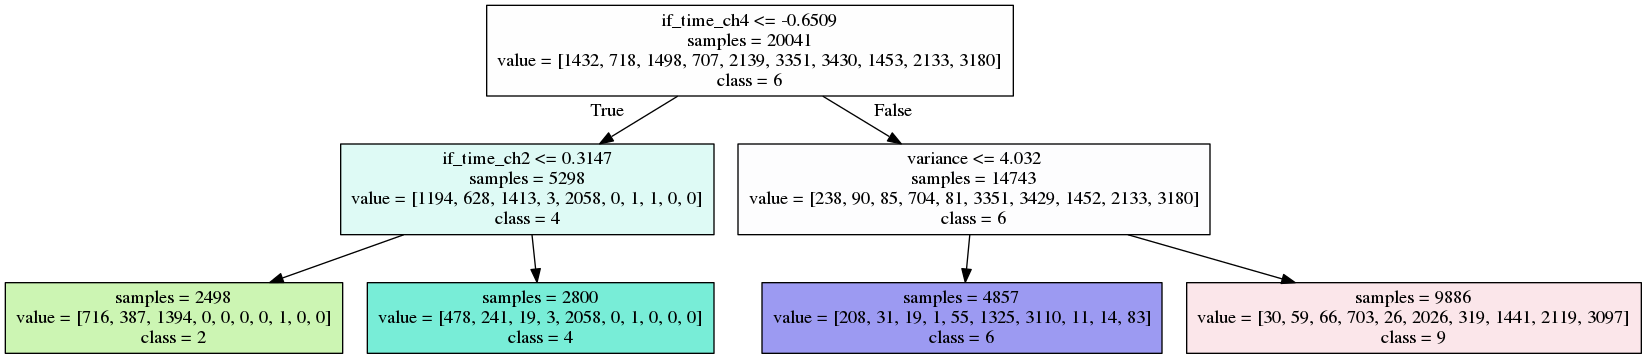
\includegraphics[width=\textwidth]{figures/dt_2}
      \caption{Extracted representation of a trained decision tree with depth=2}
      \label{fig:dt_2}
\end{figure}

    \item the \ac{SVM} do not show a clear tendency to improve as complexity is increased, and just like the K-nearest neighbor models, performs quite well in small sizes of datasets. However, the best accuracy of this model is still below the accuracies of the other models regarded in this benchmark. Additionally, the training and prediction times exceed dramatically the times achieved with the other models, being about 8000 times longer for training and around 500 times longer for prediction. The fact that this model is that slow will definitely affect considerably the performance of real-time implementations, an aspect that is crucial in systems such as cognitive radio.
\end{itemize}

\section{Scenario Classification}
Besides of the general performance that the learning models have in regard to the whole testing set, it is paramount to determine how good they perform by classifying each of the specific scenarios of Table~\ref{table:scenarios}. To assess this, confusion matrices are used to determine the number of rightfully classified scenarios, along with the false positives and false negatives. On this analysis, it is only of interest the number of correctly classified scenarios, and any misclassification affects the implementation equally, regardless of its type. Moreover, in section~\ref{ch:performance} can be seen that each algorithm behaves differently in terms not only of accuracy, but also in training time and prediction time. As the models are trained only once, the "training time" does not play a role in the model selection for this work, as it does not have any repercussion on the performance of the model when new values are applied to it. Therefore, "prediction time" and "accuracy" are metrics of quality that are considered for these models on its selection to be applied on real-time scenarios.\\

Confusion matrices show how each of the samples from the data set are classified for a given model. As a matter of illustration, a side by side comparison for the worst-performing vs. the best-performing model, with respect to accuracy, is given in Fig~\ref{fig:confusionknn}, \ref{fig:confusiondtc} and \ref{fig:confusionsvc}. The complete set of confusion matrices, corresponding to every trained model, can be found in the development notebook for this work \cite{repo:cognitive_radio_ml}.


\begin{figure}[!htb]
    \captionsetup[subfigure]{justification=centering}
    \centering
    \begin{subfigure}[htb]{0.49\textwidth}
        \centering
        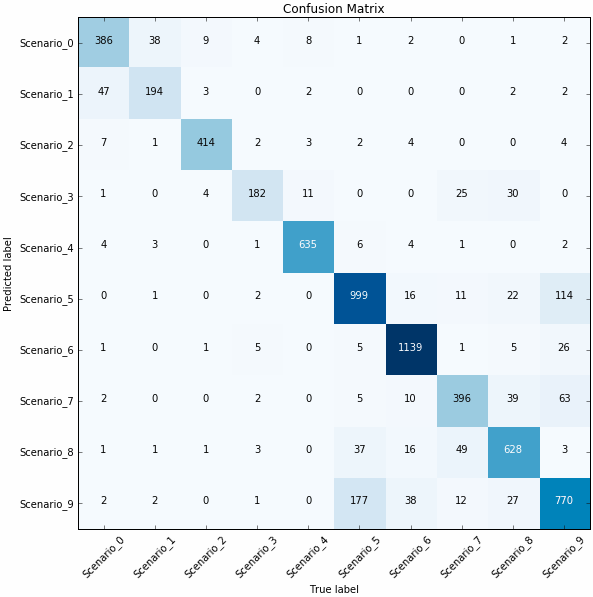
\includegraphics[width=\linewidth]{figures/knn_scaled_S_50}
        \caption{KNN-50 neighbors, StandardScaled, trained with small (S) dataset}
        \label{fig:knn_2}
    \end{subfigure}
    \begin{subfigure}[htb]{0.49\textwidth}
        \centering
        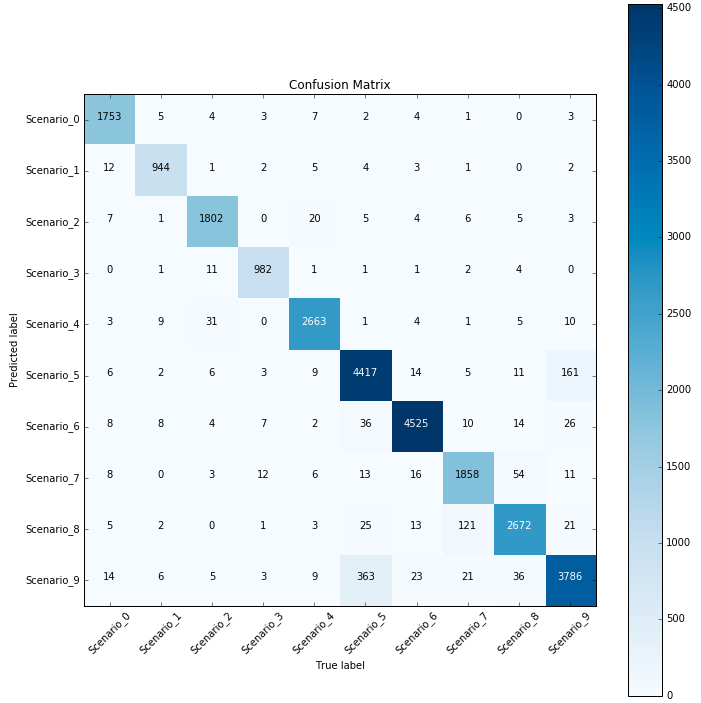
\includegraphics[width=\linewidth]{figures/knn_unscaled_XL_4}
        \caption{KNN-4 neighbors, unscaled, trained with whole (XL) dataset}
        \label{fig:knn_4}
    \end{subfigure}
    \caption{Confusion Matrixes for K-nearest Neighbor Models}
    \label{fig:confusionknn}
\end{figure}

\begin{figure}[!htb]
    \captionsetup[subfigure]{justification=centering}
    \centering
    \begin{subfigure}[htb]{0.49\textwidth}
        \centering
        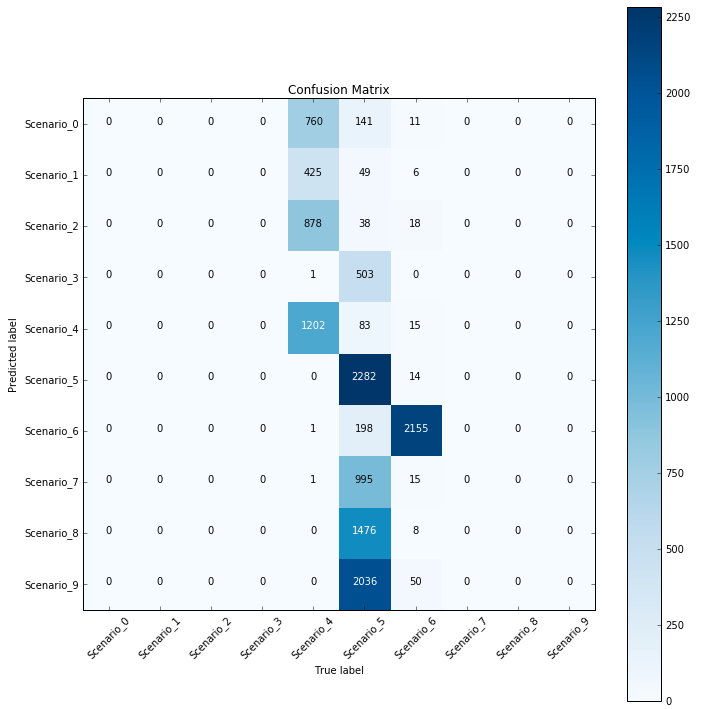
\includegraphics[width=\linewidth]{figures/dtc_unscaled_L_2}
        \caption{Decision Tree, unscaled, depth=2, trained with large (L) dataset}
        \label{fig:knn_2}
    \end{subfigure}
    \begin{subfigure}[htb]{0.49\textwidth}
        \centering
        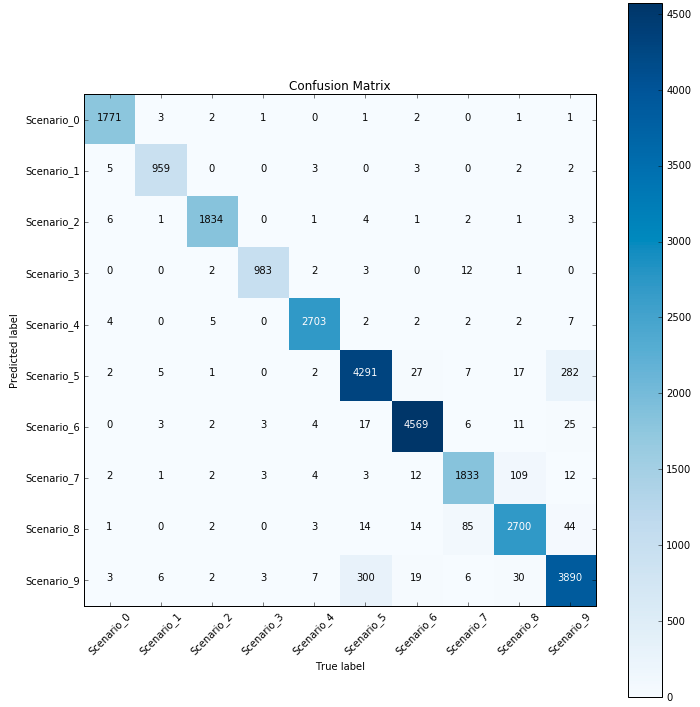
\includegraphics[width=\linewidth]{figures/dtc_unscaled_XL_50}
        \caption{Decision Tree, unscaled, depth=50, trained with whole (XL) dataset}
        \label{fig:knn_4}
    \end{subfigure}
    \caption{Confusion Matrixes for Decision Tree Models}
    \label{fig:confusiondtc}
\end{figure}
\begin{figure}[!htb]
    \captionsetup[subfigure]{justification=centering}
    \centering
    \begin{subfigure}[htb]{0.49\textwidth}
        \centering
        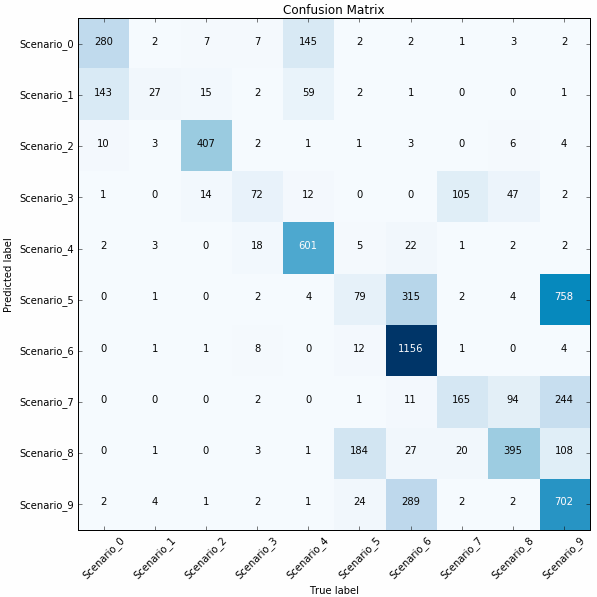
\includegraphics[width=\linewidth]{figures/svc_scaled_S_1}
        \caption{\ac{SVM}, StandardScaled, C=1, trained with small (S) dataset}
        \label{fig:knn_2}
    \end{subfigure}
    \begin{subfigure}[htb]{0.49\textwidth}
        \centering
        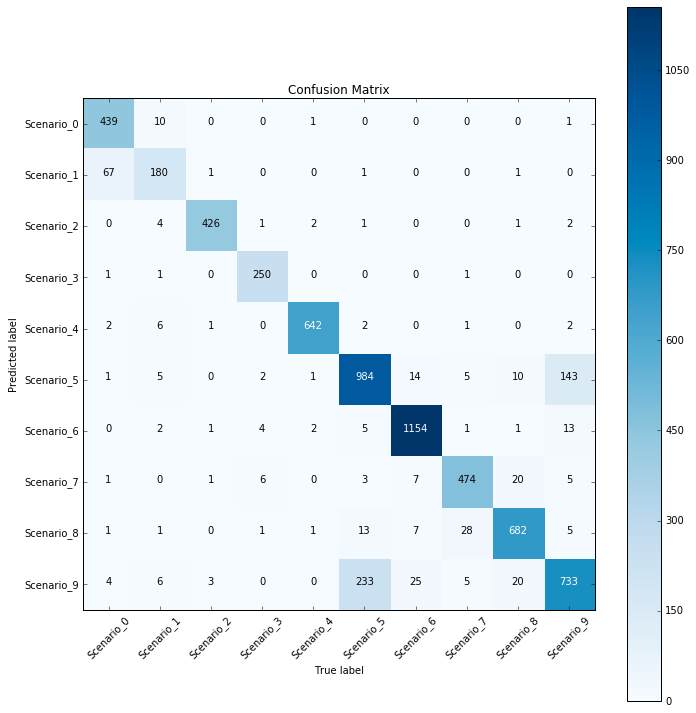
\includegraphics[width=\linewidth]{figures/svc_scaled_S_1e6}
        \caption{\ac{SVM}, StandardScaled, C=1e6, trained with small (S) dataset}
        \label{fig:knn_4}
    \end{subfigure}
    \caption{Confusion Matrixes for \ac{SVM} Models}
    \label{fig:confusionsvc}
\end{figure}
It is also important to notice the clear difference on the number of samples present for each scenario. This is due to the fact that the measurements performed in section~\ref{ch:measure} were based on runtime and not on number of generated samples, and the feature extraction algorithm described in section~\ref{ch:features} generates a different number of samples for each scenario, because of its dependence on the \emph{frame events} generation consequently of the channel occupation and interframe time of arrival itself. A different approach for feature extraction based on a number of features generated is proposed in chapter~\ref{ch:conclusions}.

From these matrices it can be clearly seen, at a first glance, that the K-Nearest algorithm performs quite well regardless of its configuration, having a more populated diagonal in its confusion matrix in comparison with the other two analyzed models. Additionally, just a small improvement in the classification accuracy is seen as the complexity and dataset size increases for this model. In general, it is safe to assert that the classification performs generally well for most of the scenarios except scenario 5, where a higher number of false positives, as well as false negatives, is seen for all models, being misclassified as scenario 9. This indicates that the extracted features for these specific scenarios have a noticeable correlation, and serve as an invitation to determine a feature that confidently sets a difference between them.
\subsection{Image Classification}\label{ch:image_classification}
For the image classification part of this work, a sequential model based on the work of \cite{Paisana2017} was implemented. The basic structure of this model is shown in Fig~\ref{fig:cnn}. As it can be seen, the model is composed of the connection of different layers, each of them with n specific functionality.

\begin{figure}[!htb]
    \centering
      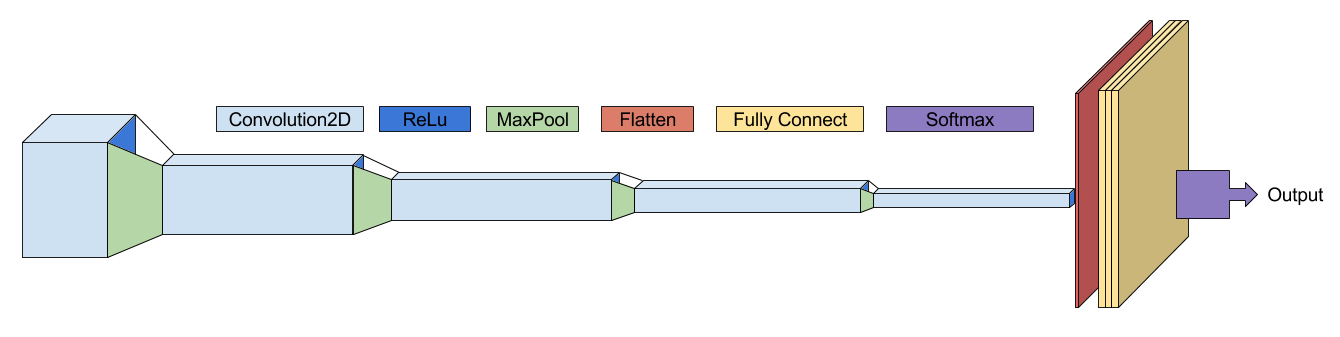
\includegraphics[width=\textwidth]{figures/cnn}
      \caption{Schema of the implemented CNN}
      \label{fig:cnn}
\end{figure}

\begin{itemize}
    \item Convolution2D: this comprises a convolutional kernel. It convolves the input to produce tensors at its output. This is the backbone of the \ac{ConvNet}, as it is the responsible for learning. Here, 2-Dimensional convolutional blocks are applied, as it is convolving over the area of the input images.
    \item MaxPool: this layer serves its purpose for dimension reduction, which is a form of downsampling. Briefly, it divides the input tensor into 2x2 non-overlapping squares and keeps the largest value present in each of these cells, effectively reducing the size of the representation, which in consequence reduces the number of parameters transitting the network. This has the effect of reducing the number of vector operations as well, making each layer of the network less processing-demandant. Additionally, as parameters are being dropped, this helps to avoid overfitting by disregarding eventual characteristics that are being "memorized". The principle of operation of such layers is shown in Fig~\ref{fig:maxpool}.
        \begin{figure}[!htb]
            \centering
              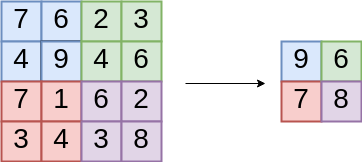
\includegraphics[width=0.4\textwidth]{figures/maxpool}
              \caption{2-D MaxPool}
              \label{fig:maxpool}
        \end{figure}
    \item \ac{ReLu}: this is an activation layer, i.e. a layer that applies a function that defines the type of output depending on its input. In the \ac{ReLu} case, the applied function is \(f(x) =\max(0,x) \), where x is the input of the neuron. Being a non-linear function, this activation increases the nonlinearity of the network without affecting the visual field, as there is no reduction of dimension.
        \begin{figure}[!htb]
            \centering
                \begin{tikzpicture}[scale=0.9]
                    \begin{axis}[
                        xlabel={$x$},
                        ylabel={$f(x)$},
                    ]
                        \addplot[domain=0.001:3,samples=201,purple,thick,smooth]{x};
                        \addplot[domain=-3:0.001,samples=201,purple,thick,smooth]{0};
                    \end{axis}
                \end{tikzpicture}
              \caption{ReLu activation function}
              \label{fig:maxpool}
        \end{figure}
    \item Fully connected layer: as the name states, this layer is connected to each one of the activations of the previous layers. These type of layers are the principle of operation of traditional neural networks, and is in charge of learning the non-linearities that have been propagated throughout the network.
    \item Softmax: this is also an activation layer. It takes vector q of dimension K and compress it together with values that add up to one. The function is given by
        \begin{equation}
            P(q)_i = \frac{e^{q_i}}{\sum_{k=1}^{K} \exp{q_j}}
        \end{equation}

        It can be easily understood that the dimension of the output from this softmax function is the number of labels to classify and that the value of each is the probability of the input sample to belong to that class. Consequently, the classification result is the \( \argmax \) of the function output.
\end{itemize}

The chosen layers and its disposition are strictly related to the input. In this case, the input picture has a 64x64 size, which describes then the height and width of the first layer. The depth is the number of filters that are used for each layer, and it is, to some extent, represented in the extension of the scale of Fig~\ref{fig:cnn}. 5 convolutional layers, with kernel dimensions 2x2, were used in this sequential model, with depths of 48, 128, 192, 192 and 128 filters correspondingly. At the end of the sequential model, 3 fully connected layers with depth 1024, 1024 and 10 were used. The sequence of dimension changes of the sequential model and the number of parameters considered in each of the stages of the classification problem is summarized in Table~\ref{table:convnet_summary}. The number of parameters is the number of trainable weights that each layer contains. For a convolutional layer, this is calculated as \( \text{\# parameters} = \text{(depth of input tensor)}\cdot\text{(depth output tensor)}\cdot\text{height}_{kernel}\cdot \text{width}_{kernel} + \text{(depth output tensor)} \). As an example, the calculation for the first layer gives:
\begin{equation*}
    1 \cdot 48 \cdot 2 \cdot 2 + 48 = 240
\end{equation*}

\begin{table}[h!]
    \centering
    \begin{tabular}{|c|c|c|}
        \hline
        \textbf{Layer} & \textbf{Output Shape} & \textbf{\# Parameters} \\
        \hline\hline
        Convolution \# 1 & (63, 63, 48) & 240 \\\hline
        ReLu \# 1 & (63, 63, 48) & 0 \\\hline
        MaxPooling \# 1 & (31, 31, 48) & 0 \\\hline
        Convolution \# 2 & (30, 30, 128) & 24704 \\\hline
        ReLu \# 2 & (30, 30, 128) & 0 \\\hline
        MaxPooling \# 2 & (15, 15, 128) & 0 \\\hline
        Convolution \# 3 & (14, 14, 192) & 98496 \\\hline
        ReLu \# 3 & (14, 14, 192) & 0 \\\hline
        MaxPooling \# 3 & (7, 7, 192) & 0 \\\hline
        Convolution \# 4 & (6, 6, 192) & 147648 \\\hline
        ReLu \# 4 & (6,6, 192) & 0 \\\hline
        MaxPooling \# 4 & (3, 3, 192) & 0 \\\hline
        Convolution \# 5 & (2, 2, 128) & 98432 \\\hline
        ReLu \# 5 & (2,2, 128) & 0 \\\hline
        MaxPooling \# 5 & (1, 1, 128) & 0 \\\hline
        flatten & 128 & 0 \\\hline
        Fully Connected \#1 & 1024 & 132096 \\\hline
        Fully Connected \#2 & 1024 & 1049600 \\\hline
        Fully Connected \#3 & 10 & 10250 \\\hline
        Softmax & 10 & 0 \\\hline
        \hline
    \end{tabular}
    \caption{ConvNet dimensions and Number of Parameters}
    \label{table:convnet_summary}
\end{table}

The sequential model performs an optimization over its error function, for which the optimizer used can be selected. Keras provides a variety of these optimizers, using the approach of the steepest descent optimization over an objective function, \(J(\theta)\) with \(\theta \in \mathbb{R}^{d}\), being \(d\) the dimension of the objective function, by updating the parameters in the opposite direction of the gradient of \(J\), i.e.

\begin{equation}
    \nabla_\theta J(\theta) \text{  w.r.t } \theta, x, y
\end{equation}

A tunable parameter is the learning rate \(\eta\), that determines the size of the steps taken to reach the minimum. For this work, three different optimizers were used and analyzed based on the resulting accuracy of the classification over the test data, as well as its value for error during validation.

\begin{itemize}
    \item Stochastic gradient descent: this algorithm performs a parameter update after each training sample
        \begin{equation}
            \theta = \theta - \eta \cdot \nabla_\theta J(\theta;x^i;y^i)
        \end{equation}
        This optimizer was used in \cite{Paisana2017} and was used as a baseline. The learning rate \(\eta\) was decreased every one-fourth of the total iterations, which in this specific use case was set to 3000. Decreasing the learning rate increases the chance that this optimizer reaches a local minimum.
    \item Adadelta \cite{Zeiler2012a}: this optimizer is based on the Adagrad optimizer \cite{Duchi2011}, which adapts intrinsically its learning rate to the parameters, therefore doing bigger updates for infrequent parameters, and smaller updates for frequent ones. It is proven that this optimizer is more robust than the stochastic gradient descent \cite{Duchi2011} by storing all previous squared gradients and updating accordingly. Adadelta extends this robustness by restricting the amount of accumulated squared gradients to a fixed window, and using this accumulation for its updates.
    \item Adamax: based on the Adaptive Moment Estimation - Adam \cite{Kingma2014}, this optimizer also sets an adaptive learning rate based on the parameters of the objective function. Additionally, to set a fixed window of past squared decays as Adadelta, Adam also keeps an exponentially decaying average of past gradients, which is similar to a momentum \cite{Dahl2013}. Adamax extends Adam functionality by maximizing the norm of the update vector, which leads to a stable behavior.
\end{itemize}

The validation of the models was performed based on the accuracy that these optimizers have during training and testing, the loss factor during the same stages, which is a measure of the error provided by the optimization process. The results are shown in Figs~\ref{fig:sgd}, \ref{fig:adamax} and \ref{fig:adadelta}.

\begin{figure}[!htb]
    \centering
    \begin{subfigure}[htb]{0.49\textwidth}
        \centering
        \begin{tikzpicture}[scale=0.8]
            \begin{axis}[
                xlabel={Iterations},
                ylabel={Loss Factor},
                  ]
                \addplot table [x=epoch, y=loss, col sep=comma, mark=none] {data/sgd.csv};
                \addplot table [x=epoch, y=val_loss, col sep=comma, mark=none] {data/sgd.csv};
                \legend{Training loss, Validation loss}
        \end{axis}
        \end{tikzpicture}
    \end{subfigure}
        \hfill
    \begin{subfigure}[htb]{0.49\textwidth}
        \centering
        \begin{tikzpicture}[scale=0.8]
            \begin{axis}[legend pos=south east,
                xlabel={Iterations},
                ylabel={Accuracy},
                  ]
                \addplot table [x=epoch, y=acc, col sep=comma, mark=none] {data/sgd.csv};
                \addplot table [x=epoch, y=val_acc, col sep=comma, mark=none] {data/sgd.csv};
                \legend{Accuracy, Validation Accuracy}
        \end{axis}
        \end{tikzpicture}
    \end{subfigure}
    \caption{Metrics for Steepest Gradient descent Optimizer}
    \label{fig:sgd}
\end{figure}


\begin{figure}[!htb]
    \centering
    \begin{subfigure}[htb]{0.49\textwidth}
        \centering
        \begin{tikzpicture}[scale=0.8]
            \begin{axis}[
                xlabel={Iterations},
                ylabel={Loss Factor},
                  ]
                \addplot table [x=epoch, y=loss, col sep=comma, mark=none] {data/adamax.csv};
                \addplot table [x=epoch, y=val_loss, col sep=comma, mark=none] {data/adamax.csv};
                \legend{Training loss, Validation loss}
        \end{axis}
        \end{tikzpicture}
    \end{subfigure}
        \hfill
    \begin{subfigure}[htb]{0.49\textwidth}
        \centering
        \begin{tikzpicture}[scale=0.8]
            \begin{axis}[legend pos=south east,
                xlabel={Iterations},
                ylabel={Accuracy},
                  ]
                \addplot table [x=epoch, y=acc, col sep=comma, mark=none] {data/adamax.csv};
                \addplot table [x=epoch, y=val_acc, col sep=comma, mark=none] {data/adamax.csv};
                \legend{Accuracy, Validation Accuracy}
        \end{axis}
        \end{tikzpicture}
    \end{subfigure}
    \caption{Metrics for Adamax Optimizer}
    \label{fig:adamax}
\end{figure}

\begin{figure}[!htb]
    \centering
    \begin{subfigure}[htb]{0.49\textwidth}
        \centering
        \begin{tikzpicture}[scale=0.9]
            \begin{axis}[
                xlabel={Iterations},
                ylabel={Loss Factor},
                  ]
                \addplot table [x=epoch, y=loss, col sep=comma, mark=none] {data/adadelta.csv};
                \addplot table [x=epoch, y=val_loss, col sep=comma, mark=none] {data/adadelta.csv};
                \legend{Training loss, Validation loss}
        \end{axis}
        \end{tikzpicture}
    \end{subfigure}
    \hfill
    \begin{subfigure}[htb]{0.49\textwidth}
        \centering
        \begin{tikzpicture}[scale=0.9]
            \begin{axis}[legend pos=south east,
                xlabel={Iterations},
                ylabel={Accuracy},
                  ]
                \addplot table [x=epoch, y=acc, col sep=comma, mark=none] {data/adadelta.csv};
                \addplot table [x=epoch, y=val_acc, col sep=comma, mark=none] {data/adadelta.csv};
                \legend{Accuracy, Validation Accuracy}
        \end{axis}
        \end{tikzpicture}
    %}
    \end{subfigure}
    \caption{Metrics for Adadelta Optimizer}
    \label{fig:adadelta}
\end{figure}

From these plots, it can clearly be seen that SGD takes a greater number of iterations to reach its maximum accuracy as well as its minimum loss factor in comparison with Adamax and Adadelta. With respect to their comparative accuracies, it is not conclusive that one of the optimizers provide a better result. The maximum and final values of the accuracies of these models are shown in Table~\ref{table:convnet_accs}, whilst the minimum and final values for the loss factor are shown in Table~\ref{table:convnet_loss}.

\begin{table}[!ht]
  \centering
    \begin{tabular}{| >{\centering\arraybackslash}m{5em}| >{\centering\arraybackslash}m{7em}| >{\centering\arraybackslash}m{7em}| >{\centering\arraybackslash}m{7em}| >{\centering\arraybackslash}m{7em}|}
    \cline{2-5}
      \multicolumn{1}{c|}{} & Max Training Accuracy (Iter) & Final Training Accuracy & Max Validation Accuracy (iter) & Final Validation accuracy \\ \hline
      SGD & 99\% (2411)   & 98\%   & 90\% (981) & 81\%  \\ \hline
      Adamax & 92\% (2997)   & 88\%   & 87\% (2679) & 77\%  \\ \hline
      Adadelta & 100\%(2012)   & 99.6\%   & 89\% (489) & 85\%  \\ \hline
  \end{tabular}
    \caption{Maximum and Final Accuracies for ConvNets with various optimizers}
    \label{table:convnet_accs}
\end{table}


\begin{table}[!ht]
  \centering
    \begin{tabular}{| >{\centering\arraybackslash}m{5em}| >{\centering\arraybackslash}m{7em}| >{\centering\arraybackslash}m{7em}| >{\centering\arraybackslash}m{7em}| >{\centering\arraybackslash}m{7em}|}
    \cline{2-5}
      \multicolumn{1}{c|}{} & Min Training Loss (Iter) & Final Training Loss & Min Validation Loss (iter) & Final Validation Loss \\ \hline
  SGD & 0.625 (2866)   & 0.64   & 0.863 (861) & 1.134  \\ \hline
      Adamax & 0.24 (2997)   & 0.37   & 0.47 (1150) & 0.93  \\ \hline
      Adadelta & 0.03 (2998)   & 0.04   & 0.4 (297) & 0.74  \\ \hline
  \end{tabular}
    \caption{Maximum and Final Loss Factor for ConvNets with various optimizers}
    \label{table:convnet_loss}
\end{table}

The low values for losses as well as high values for accuracies in the training process do not come as a surprise, but it is the iteration where they are reached what is significant to be analyzed, as they state the rate of convergence of each of the optimizers. For the training phase, it is also expected that these values are constantly increasing along the whole process, as the model keeps learning from the data and fits to it. Therefore, it is of special interest to focus the attention to the validation part. Regarding the accuracy value, it is not conclusive to determine an algorithm that outperforms the others. Additionally, an accuracy greater than 87\% for all the optimizers is satisfactory, keeping in mind that these models are trained with spectrograms with SNR as low as -5dB, where the \ac{PU} signal is well below the noise level. It is clear that the rate of convergence of Adadelta surpasses the performance of the other optimizers, for both the maximum validation accuracy and the minimum validation loss, which states that using early stop techniques allows having a satisfactory model with short training time. More insights about the early stop techniques are given in the following chapter, where it will be clear why the maximum validation accuracy and minimum validation loss are important values to be considered.

Looking carefully at the loss factor plots for validation, a clear tendency of the increase of this parameter at the end of the iterative process can be seen for the Adamax and Adadelta optimizers, which is an indication of overfitting. Although not clear from the plots, SGD also shows overfitting behavior to some extent, as it can be seen in the noticeable difference on the maximum accuracy vs the final accuracy in table~\ref{table:convnet_accs}.

